\documentclass{article}
\usepackage[utf8]{inputenc}
\usepackage{geometry}
\geometry{margin = .25in}
\usepackage{amsmath, amsthm, amssymb, enumitem, graphicx}
\graphicspath{ {images/} }
\usepackage{etoolbox}
\newtheorem{problem}{Problem}
\theoremstyle{definition}
\newtheorem*{solution}{Solution}

\begin{document}

\title{Math 240 (Discrete Structures 1) Assignment 2}
\author{Victoria Pittard, ID 260762268}
\date{\today}

\maketitle

%%Problem 1
\begin{problem}
\textbf{Negation of Predicates:} for each of the sentences below,
\begin{itemize}
    \item write it using symbolic logic notation, using the indicated predicates;
    
    \item find the negation of your sentence from (i) and simplify as much as possible; and
    
    \item re-write your answer from (ii) in English (with appropriate mathematical notation where applicable). Your answer should match the one from (ii) exactly; answers which differ will not receive full marks, even if logically equivalent.
\end{itemize}

\begin{enumerate}[label = \alph*)]
    \item Something is rotten in the state of Denmark. [D(x): x is in Denmark; R(x): x is rotten]
    
    \item For every real number $\epsilon > 0$ there is a positive real number N such that $x>N$ implies that $|f(x)-L|<\epsilon$. [B(x,y): $x>y$]
\end{enumerate}
\end{problem}

\begin{solution}
\end{solution}

\begin{enumerate}[label = \alph*)]
    \item
    
    \begin{enumerate}[label = \alph*.]
        \item
        $\exists x (D(x) \wedge R(x))$
        \item 
        \begin{align*}
            \neg(\exists x(D(x)\wedge R(x)) &\equiv \forall x \neg (D(x) \wedge R(x)) &\text{(Negation)} \\
            &\equiv \forall x(\neg D(x) \vee \neg R(x)) &\text{(DeMorgan's)}
        \end{align*}
        \item For all x, either x is not in Denmark or x is not rotten.
    \end{enumerate}
    
    \item
    \begin{enumerate}[label = \alph*)]
        \item
        $(\epsilon > 0) \implies \forall \epsilon (\exists N(B(N,0)\wedge(B(x,N)) \implies B(\epsilon , |f(x)-L|)))$
        
        \item
        \begin{align*}
            &\equiv\neg((\epsilon > 0) \implies \forall \epsilon (\exists N(B(N,0)\wedge(B(x,N)) \implies B(\epsilon , |f(x)-L|))))&\text{(Negation)} \\
            &\equiv (\epsilon>0) \wedge \neg(\forall \epsilon(\exists N(B(N,0)\wedge B(X,N))\implies B(\epsilon, \mid f(x)-L \mid ))) &\text{(Conditional)}\\
            &\equiv (\epsilon >0) \wedge \neg(\forall \epsilon (\exists N \neg (B(N,0) \wedge B(X, N)) \vee B (\epsilon, \mid f(x)-L))) &\text{(Conditional)}\\
            &\equiv (\epsilon >0) \wedge \exists \epsilon (\forall N \neg((\neg (B(N,0) \wedge B(X,N)) \vee B(\epsilon, \mid f(x)-L\mid )))) &\text{(Negation 2x)}\\
            &\equiv (\epsilon >0) \wedge \exists \epsilon (\forall N \neg (\neg B(N,0)) \wedge \neg (\neg B(X,N)) \wedge \neg B(\epsilon, \mid f(x) - L \mid )) &\text{(DeMorgan's 2x)}\\
            &\equiv (\epsilon >0) \wedge \exists \epsilon (\forall N(B(N,0) \wedge B(X,N) \wedge \neg B(\epsilon, \mid f(x)-L\mid ))) &\text{(Double Neg)}
            -
        \end{align*}
        
        \item
        There exists a number $\epsilon > 0$ such that for all numbers N, x is greater than N and $\epsilon$ is not greater than f(x)-L
    \end{enumerate}
\end{enumerate}

%%problem 2
\begin{problem}
\textbf{Rules of Inference:} 
\begin{enumerate}[label = \alph*)]
    \item Verify the transitivity inference rule using a truth table (do not just give the table, but also clearly state why your table shows the argument is valid).
    
    \item Verify the modus tollens inference rule by showing an appropriate statement is a tautology.
    
    \item Use the rules of inference given on the handout to determine if the following argument is valid. Clearly state which rules you are using (you may symbolize if it is helpful).
    \begin{center}
        \begin{tabular}{l c}
             If I study, then I will pass\\
             If I do not go to a movie, then I will study. \\
             I did not pass. \\ \hline
             Therefore, I went to a movie.
        \end{tabular}
    \end{center}
\end{enumerate}
\end{problem}

\begin{solution}
\end{solution}
\begin{enumerate}[label = \alph*)]
    \item
    \begin{tabular}{|c|c|c|c|c|c|c|c|}
         \hline
         P & Q & R & $\neg P \vee Q$ & $\neg Q \vee R$ & $\neg P \vee R$ & $(\neg P \vee Q) \wedge (\neg Q \vee R)$ & $((\neg P \vee Q) \wedge (\neg Q \vee R)) \implies (\neg P \vee R)$\\ \hline
         T & T & T & T & T & T & T & T \\ \hline
         T & T & F & T & F & F & F & T \\ \hline 
         T & F & T & F & T & T & F & T \\ \hline
         T & F & F & F & T & F & F & T \\ \hline
         F & T & T & T & T & T & T & T \\ \hline
         F & T & F & T & F & T & F & T \\ \hline
         F & F & T & T & T & T & T & T \\ \hline
         F & F & F & T & T & T & T & T \\ \hline 
    \end{tabular}
    \\
    The transitivity inference rule states that if P implies Q and Q implies R, then P implies R $((P\implies Q) \wedge (Q \implies R)) \implies (P \implies R)$. $P\implies Q$, $Q \implies R$, and $P\implies R$ can be simplified to $\neg P \vee Q$, $\neg Q \vee R$, and $\neg P \vee R$ (respectively) using the conditional identity, thus the truth table tests the validity of the transitivity inference rule.
    
    \item
    The Modus Tollens inference rule can be written as $((P\implies Q) \wedge \neg Q) \implies \neg P$
    \begin{align*}
        ((P\implies Q) \wedge \neg Q) \implies \neg P &\equiv \neg ((P\implies Q) \wedge \neg Q) \vee \neg P &\text{(Conditional)}\\ 
        &\equiv (\neg P \wedge \neg Q) \vee (Q \wedge \neg Q) \implies \neg P &\text{(Distributive)}\\
        &\equiv (\neg P \wedge \neg Q) \vee F \implies \neg P &\text{(Complement)}\\
        &\equiv (\neg P \wedge \neg Q) \implies \neg P &\text{(Identity)}\\
        &\equiv \neg (\neg P \wedge \neg Q) \vee \neg P &\text{(Complement)}\\
        &\equiv (P \vee Q) \vee \neg P &\text{(DeMorgan's)}\\
        &\equiv (P \vee \neg P) \vee Q &\text{(Commutative, Associative)}\\
        &\equiv T \vee Q &\text{(Complement)}\\
        &\equiv T &\text{(Domination)}
    \end{align*}
    \\Thus, Modus Tollens is a tautology (always true).
    
    \item
    Let "I study" be represented by S, I pass be represented by P, and I go to a movie be represented by M: \\
    The argument may now be rewritten:\\
    \begin{tabular}{l}
         $S\implies P$\\
         $\neg M \implies S$\\
         $\neg P$ \\ \hline
         $\therefore M$
    \end{tabular}
    
    \begin{tabular}{|c c|c|}
        \hline
         1. & $S\implies P$ & Premise \\ \hline
         2. & $\neg P$ & Premise \\  \hline
         3. & $\neg S$ & Modus Tollens (1, 2) \\ \hline
         4. & $\neg M \implies S$ & Premise \\ \hline
         5. & $M$ & Modus Tollens (4, 5) \\ \hline
    \end{tabular}
\end{enumerate}

%%problem 3
\begin{problem}
\textbf{Set Operations:} Let $A=\{n\in \mathbb{N}$ $|$ $n<7\}, B=\{q\in \mathbb{Q}$ $|$ $|x-2| -1)\}, C = \{r\in \mathbb{R}$ $|$ $r^3-r=0$\}, and $D = \{1,2,\{1, 2\}\}$. Find each of the following (recall $\mathcal{P}(X)$ denotes the power set of X). Do not use "..." in your answer; give clear rules for set membership if you need them.
\begin{enumerate}[label = \alph*)]
    \item A $\oplus$ C
    
    \item A $\cap$ D
    
    \item C $\cup$ D
    
    \item $\{1, \{2\} \} \cup D$
    
    \item $B \setminus (A \oplus C)$
    
    \item $\{ \emptyset \} \setminus \mathcal{P}(A)$
    
    \item $(A \setminus B) \setminus (C \setminus \overline{D})$
    
    \item $\mathcal{P}(D) \cap D$
    
    \item $A \cap (\overline{B \cup C})$
    
\end{enumerate}
\end{problem}

\begin{solution}
\end{solution}
\begin{enumerate}[label = \alph*)] 
    \item 
    A includes 1, 2, 3, 4, 5, 6\\
    Of these values, C only includes 1 $(1^3-1=0)$\\
    $A\oplus C$ includes the values that are in A or C, but not both\\
    $\therefore A\oplus C = \mathbf{\{2, 3, 4, 5, 6\}}$
    
    \item
    A includes 1, 2, 3, 4, 5, 6\\
    D includes 1, 2, \{1,2\}\\
    $A\cap D$ includes the values that exist in both A and D\\
    $\therefore A\cap D = \mathbf{\{1, 2\}}$
    
    \item
    D includes 1, 2, \{1,2\}\\
    Of these values, C only includes 1 $(1^3-1=0)$\\
    $C\cup D$ includes values that are in C, D, or both\\
    $\therefore C\cup D = \mathbf{\{\{1,2\}, 2, r \in \mathbb{R} \mid r^3 - r = 0\}} $
    
    \item
    D includes 1, 2, \{1,2\} \\
    $\{1, \{2\}\} \cup D$ includes values that are in D, the indicated set, or both\\
    $\therefore \{1, \{2\}\} \cup D = \mathbf{\{1, 2, \{2\}, \{1, 2\}\}}$
    
    \item
    As shown in question 3a, $A\oplus C = \{2, 3, 4, 5, 6\}$\\
    $B \setminus (A \oplus C)$ includes the values in B, but not in $A\oplus C$\\
    $\therefore B\setminus (A\oplus C) = \mathbf{\{q \in \mathbb{Q} \mid \mid q-2\mid <1, q<2 or q>6\}}$
    
    \item
    $\{\emptyset\}$ only contains $\emptyset$\\
    The power set of A also includes $\emptyset$\\
    $\therefore \{\emptyset\}\setminus\mathcal{P}(A) = \{\}$
    
    \item
    $C\setminus \overline{D}$ consists of elements in C and D (only 1 satisfies this condition)\\
    $A\setminus B$ consists of elements in A but not in B\\
    The only element in A that is also in B is 2, thus $A\setminus B$ includes 1, 3, 4, 5, and 6\\
    Thus, this set includes the elements in A$\setminus$B but not in C$\setminus\overline{D}$ (1, 3, 4, 5, 6) minus (1)\\
    $\therefore (A\setminus B)\setminus (C\setminus \overline{D}) = \mathbf{\{3,4,5,6\}}$
    
    \item
    $\mathcal{P}(D) = \{\{1\}, \{2\}, \{\emptyset\}, \{1, 2\}, \{1, 2, \{1,2\}\}, \{11,\{1,2\}\}, \{2,\{1,2\}\}\}$\\
    $\mathcal{P}(D) \cap D$ includes the elements in D and $\mathcal{P}(D)$\\
    $\therefore \mathbf{\mathcal{P}(D) \cap D = \{\{1\}, \{2\}, \{1,2\}, \emptyset\}}$
\end{enumerate}

%%problem 4
\begin{problem}
\textbf{Venn Diagrams:} Draw a Venn Diagram for each of the following. You may include graphics for your diagrams.
\begin{enumerate}[label = \alph*)]
    \item $A \cap (\overline{B \cup C})$
    
    \item $\overline{A} \setminus (B \cup \overline{C})$

    \item $(A \cup B) \oplus (C \setminus B)$
\end{enumerate}
\end{problem}

\begin{solution}
\end{solution}

\begin{enumerate}[label = \alph*)]
    \item 
    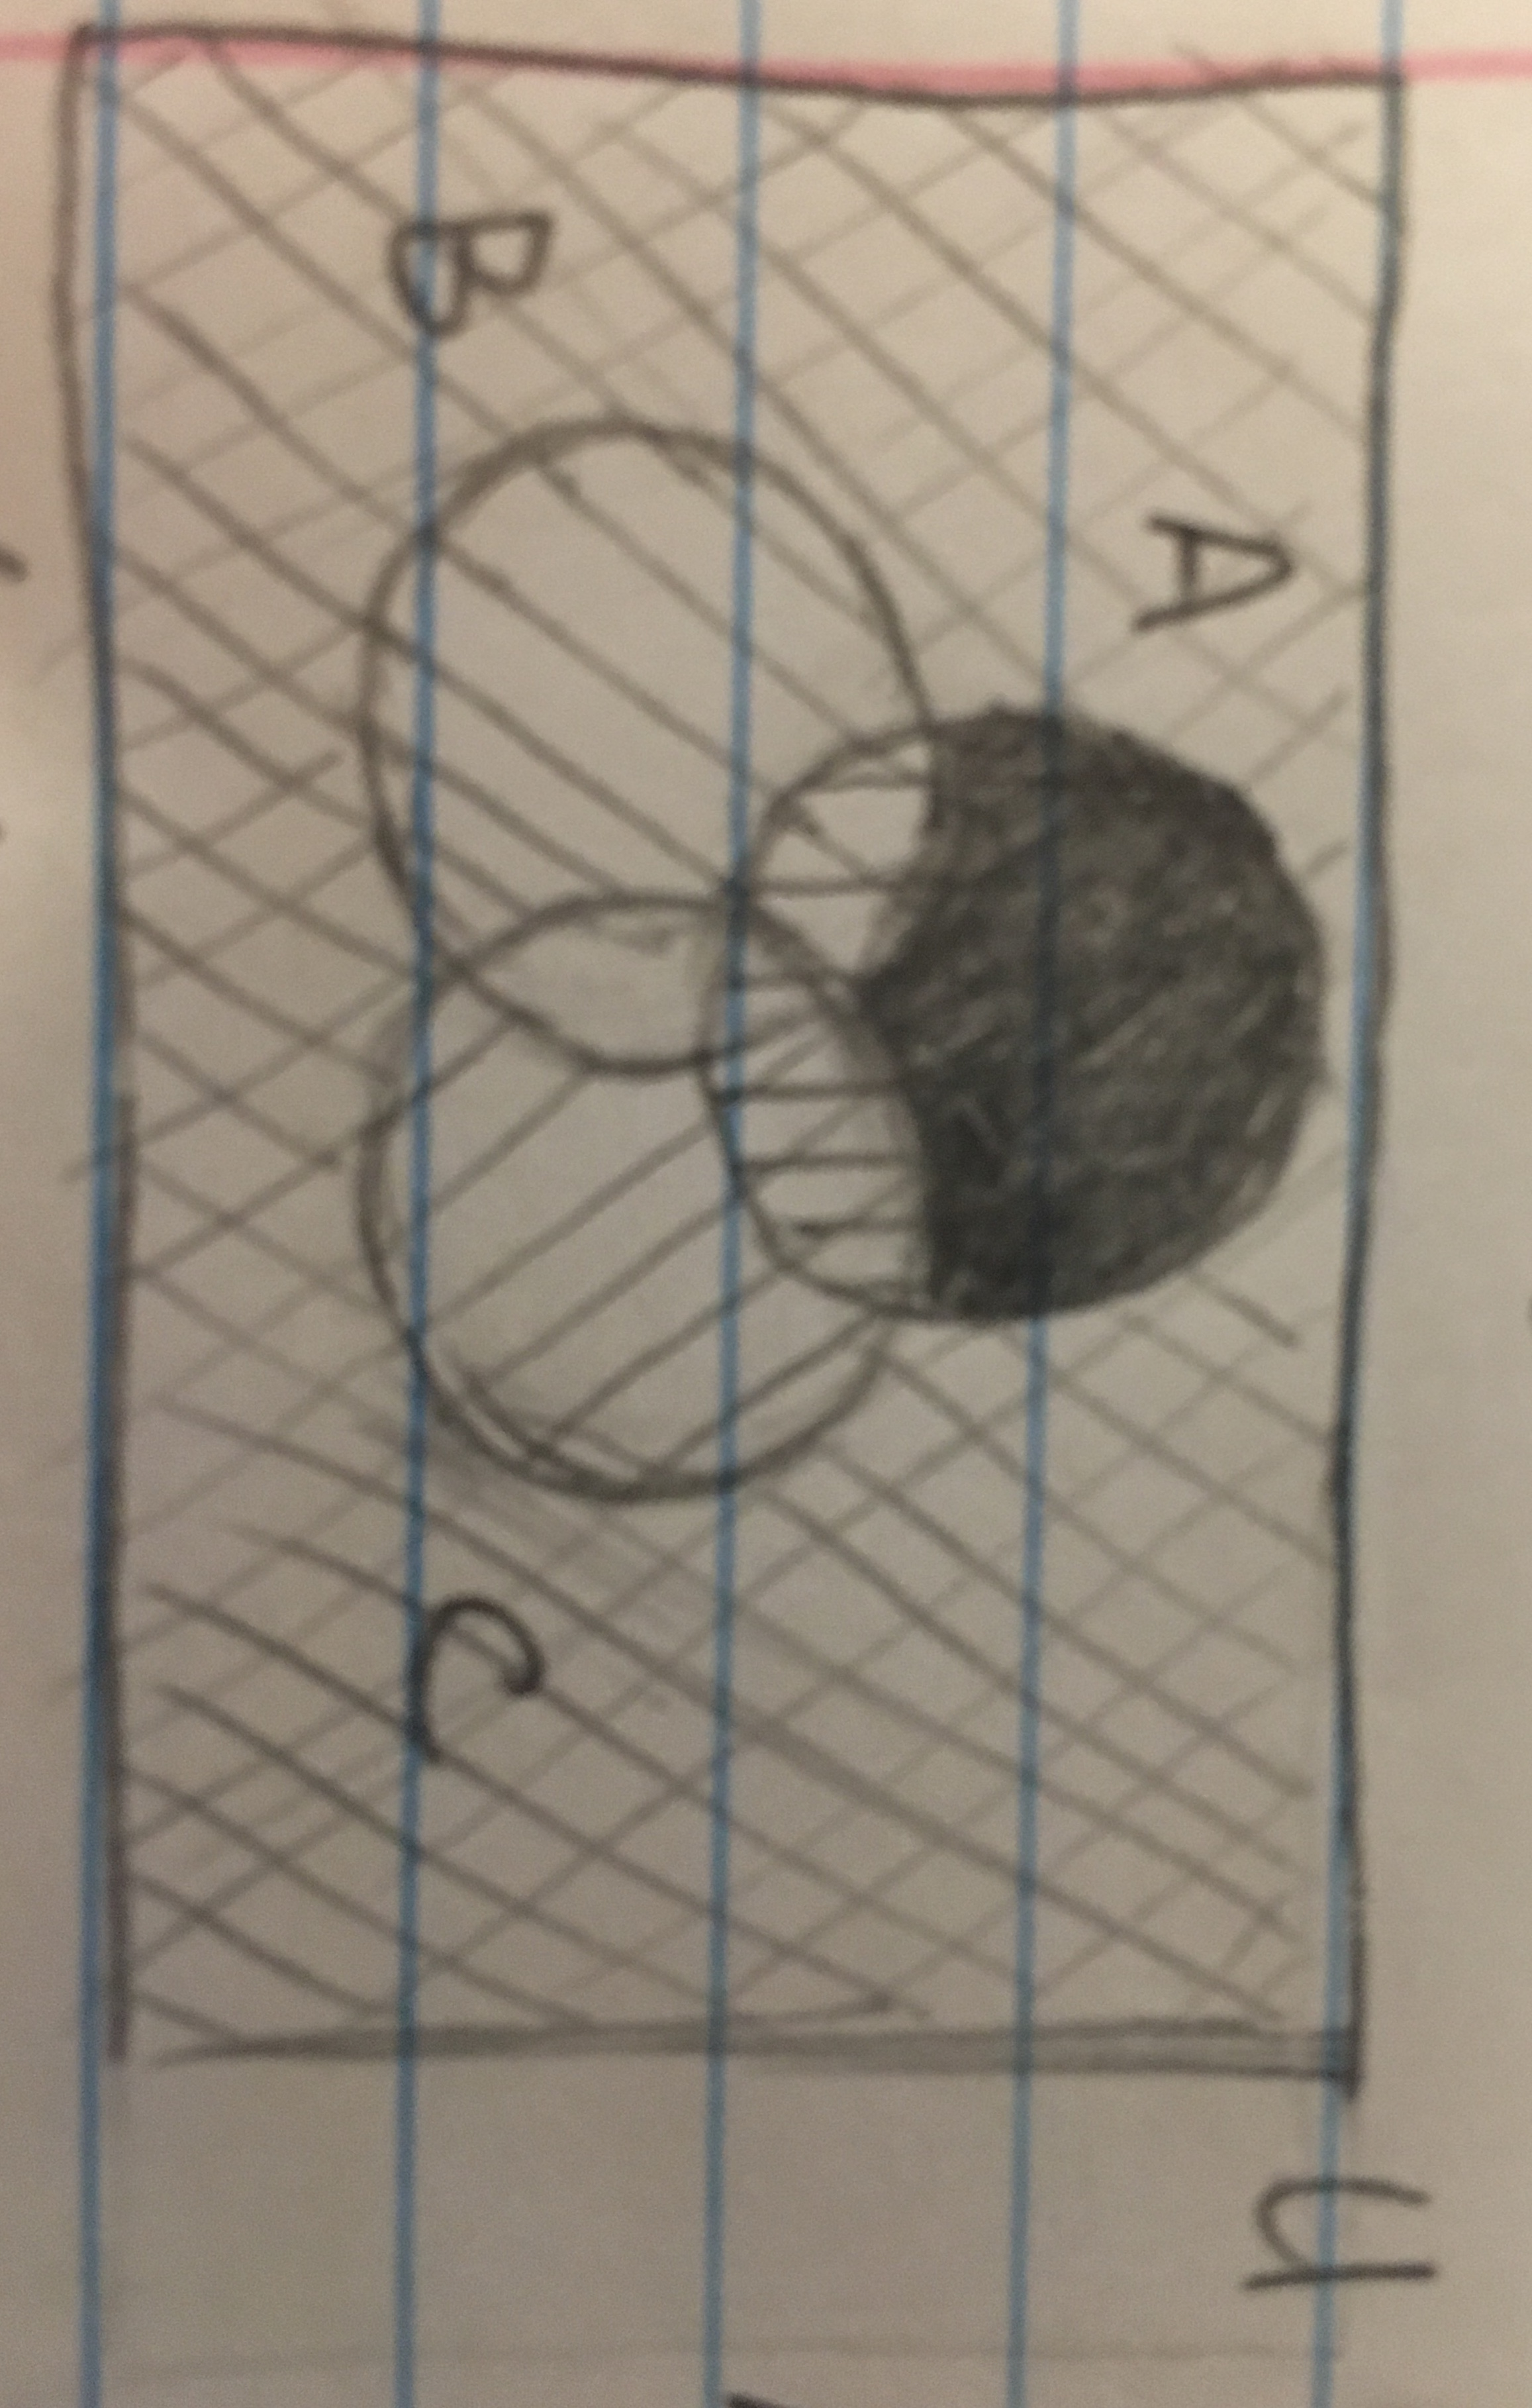
\includegraphics[scale = .045, angle = 90]{partA}
    
    \item
    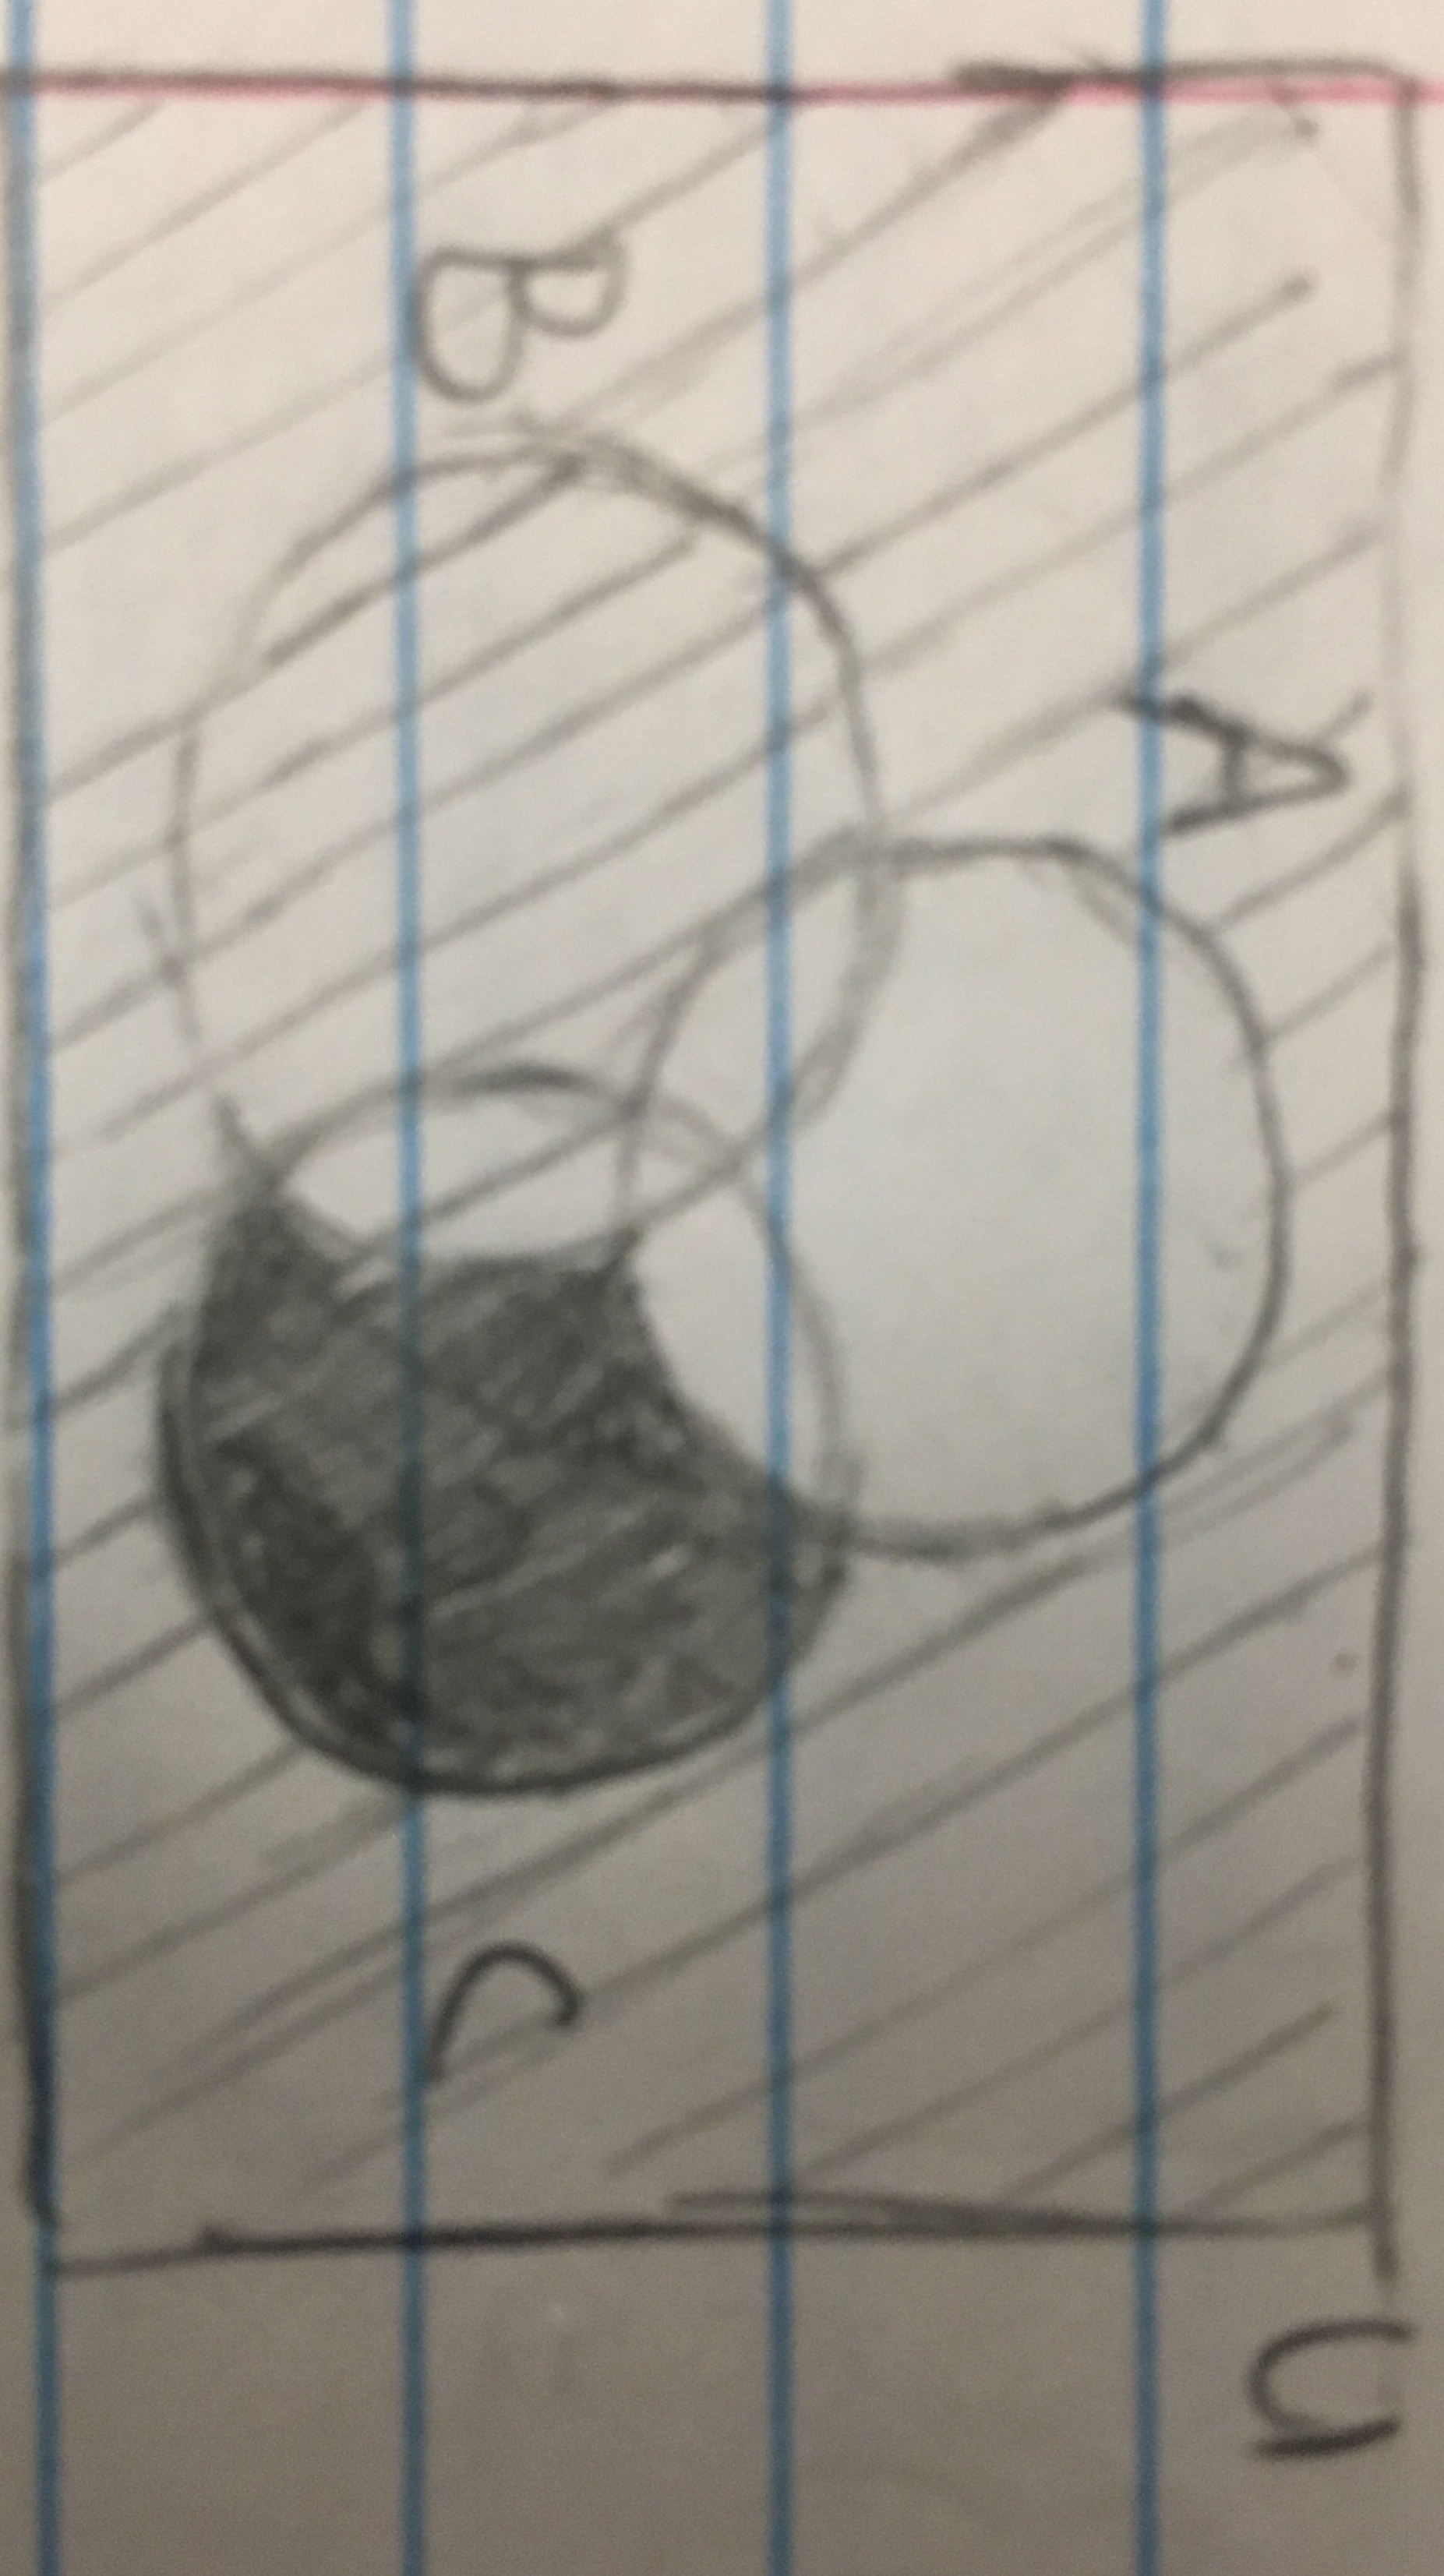
\includegraphics[scale = .05, angle = 90]{partB}
    
    \item
    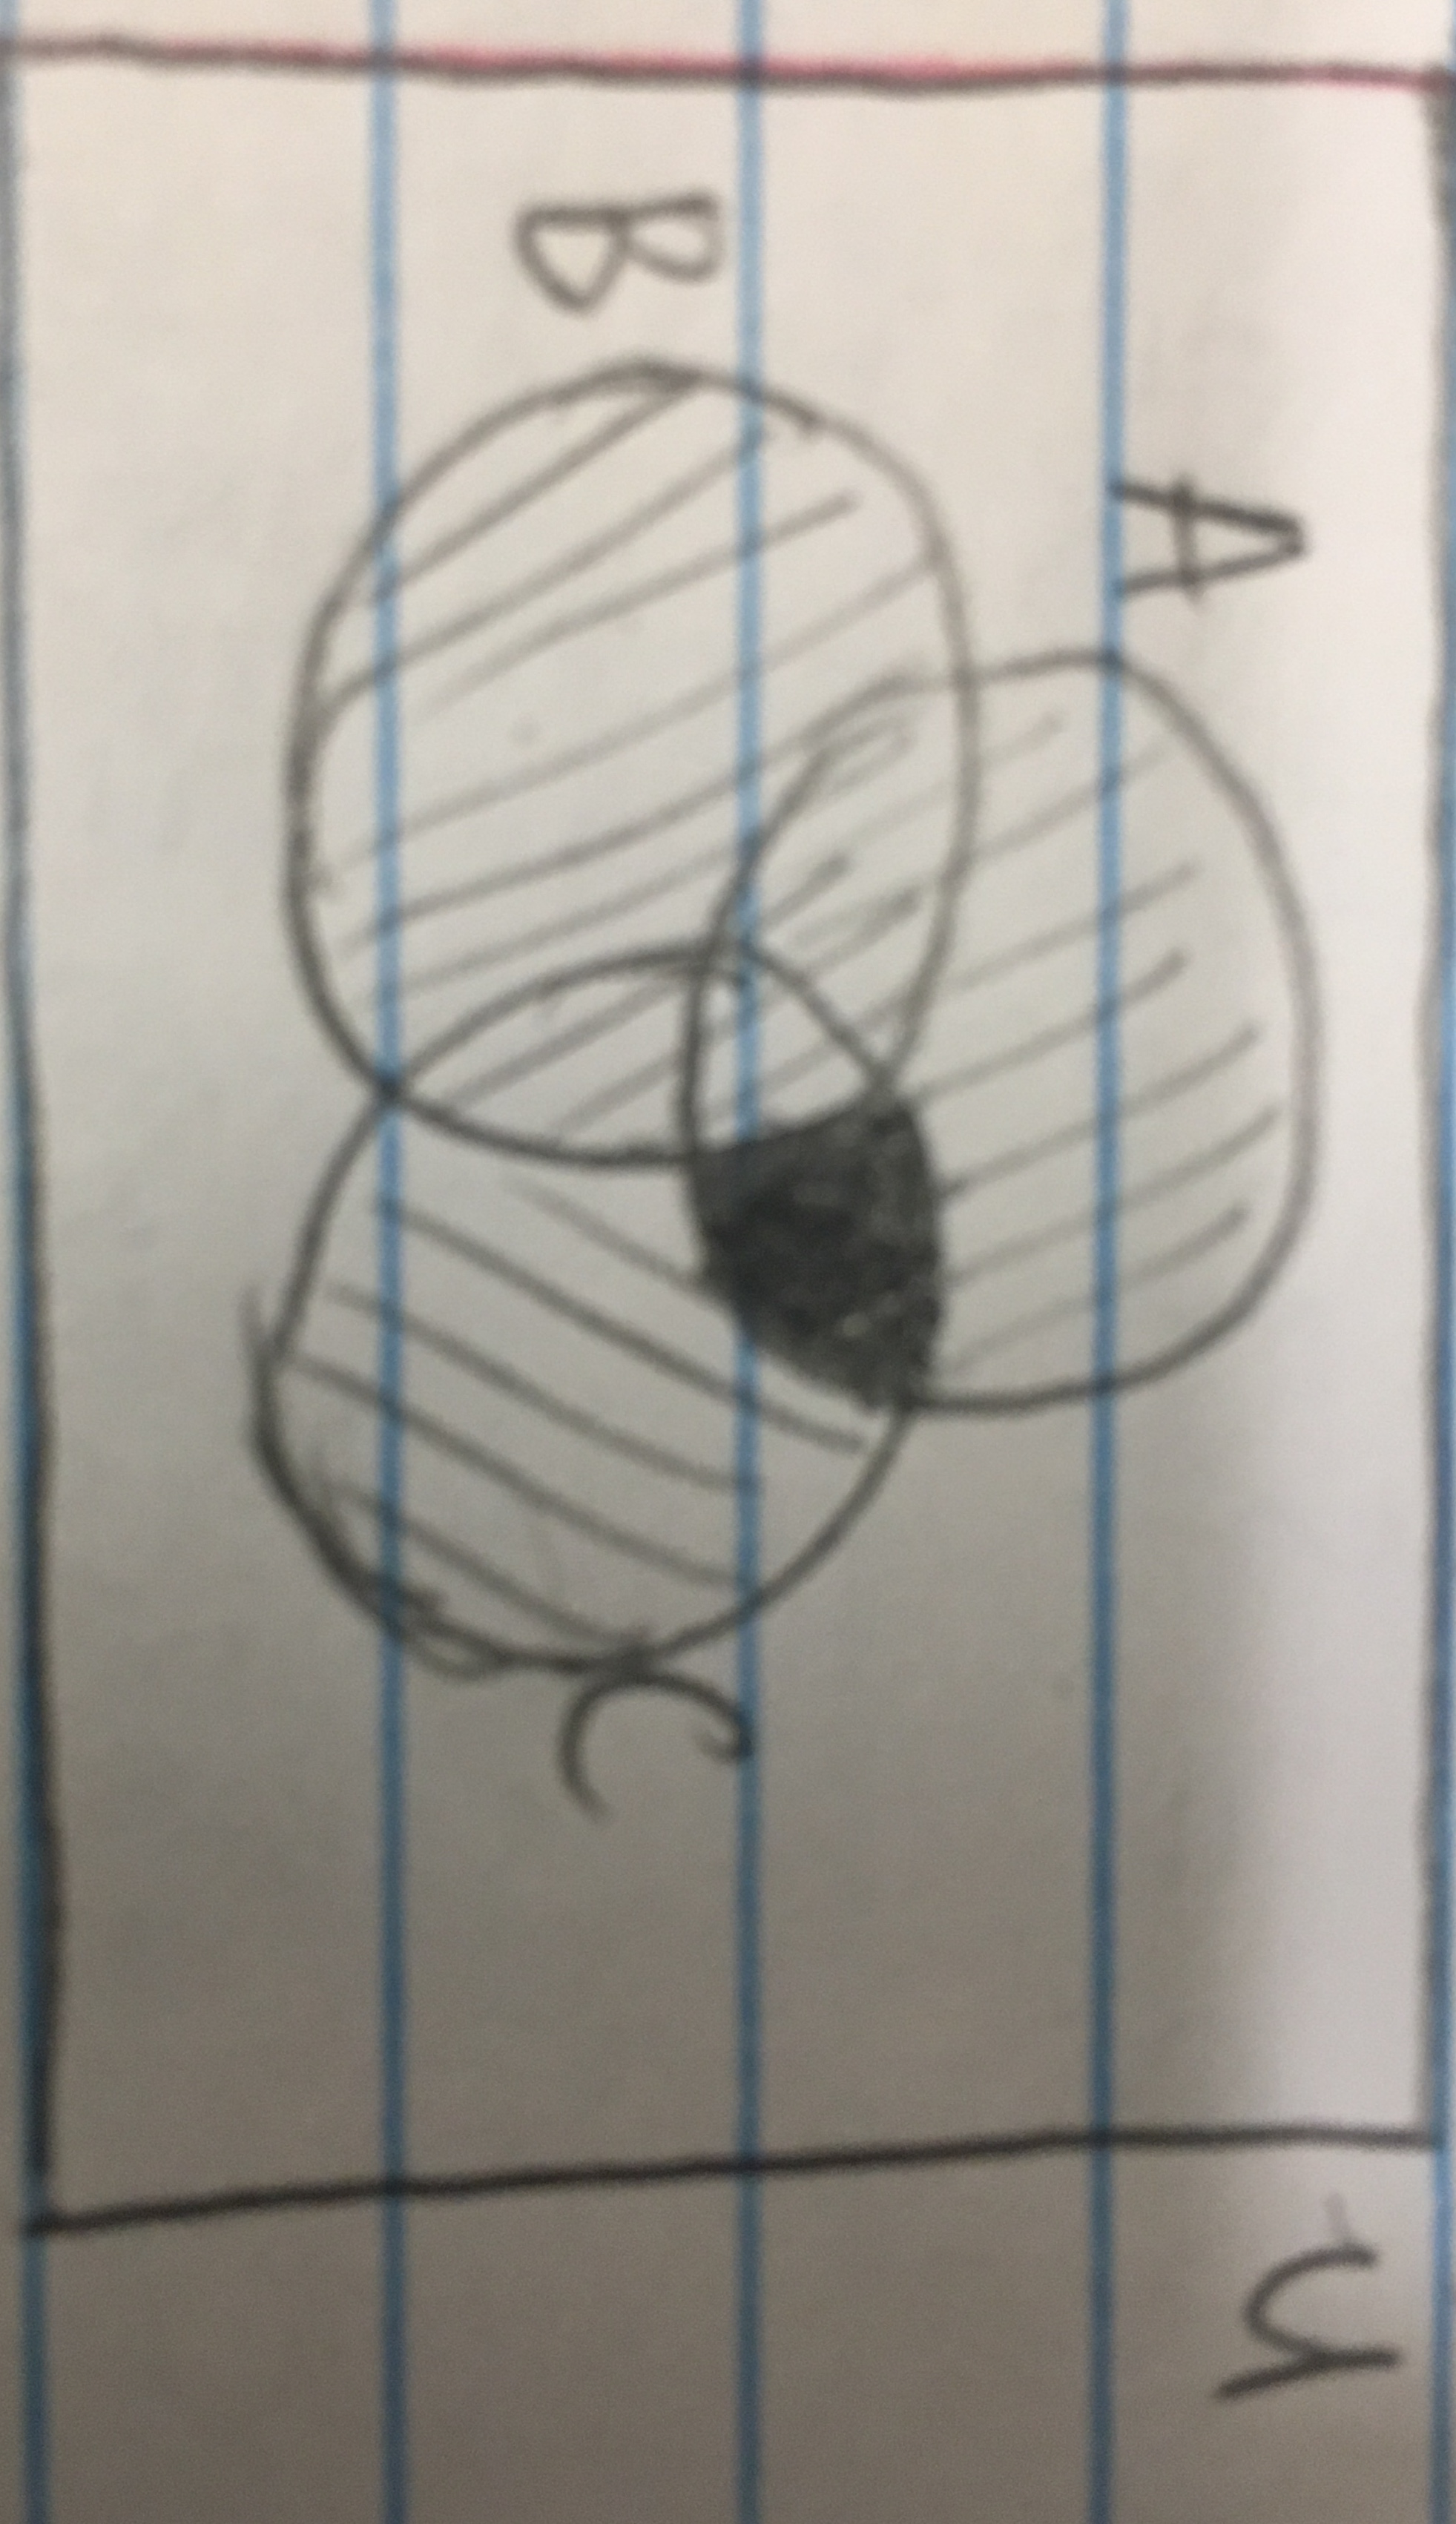
\includegraphics[scale = .05, angle = 90]{partC}
\end{enumerate}
\end{document}